\documentclass[fullscreen=true, unicode, bookmarks=false]{beamer}

\usepackage{lmodern}

\usepackage[T2A]{fontenc} 
\usepackage[cp1251]{inputenc}
\usepackage[russian]{babel}
\usepackage{amsmath,amsfonts,amssymb}
\usepackage[export]{adjustbox}
\usepackage{textgreek}
\sloppy

\setbeamertemplate{navigation symbols}{}

\usetheme{Madrid}

\usecolortheme{whale}

\usefonttheme{professionalfonts} % default family is serif

\setbeamertemplate{footline}{\hspace*{.5cm}\scriptsize{\insertshorttitle
\hspace*{50pt} \hfill\hspace*{.5cm}}\vspace{5pt}} 

\setbeamercolor{bibliography entry author}{fg=black}

\title[]{ The loss of stability for null solution in parabolic boundary-value problem with the deviate in edge condition }   
\author[]{{\large Leonid Ivanovsky}} 
\date{}
\institute[]
{ postgraduate student }

\titlegraphic{
   
\includegraphics[scale = 0.48]{yarsu_logo.png}
}

\begin{document}

\begin{frame}
\titlepage
\end{frame} 

\begin{frame}
\frametitle{ Parabolic boundary-value problem }
 
\begin{equation}\label{ivanovsky-eq1}
	u' = d \ddot{u} - \gamma u + F(u),
\end{equation}	
	
$$  u'\mid_{x=0} \, = 0, $$
$$ u'\mid_{x=1} \, = \alpha\,u\mid_{x=x_0}. $$

$$ \alpha, \gamma \in \mathbb{R}, \quad d > 0, \quad x_0 \in [0, 1]. $$

\end{frame}

\begin{frame}
\frametitle{ Substitutions }
	
$$ t_1 = dt, $$

\bigskip

$$ u(x, t) = w(x)\,\mbox{exp}\left( \lambda - \frac{\gamma}{d}t \right). $$

\end{frame}

\begin{frame}
\frametitle{ Simplified parabolic boundary-value problem }
	
\begin{equation}\label{ivanovsky-eq2}
	w'' - \lambda w = 0,
\end{equation}

$$ w'(0) = 0, $$
$$ w'(1) = \alpha\,w(x_0). $$

\end{frame}

\begin{frame}
\frametitle{ Deviate in edge condition }
	
$$ x_0 = 0: $$

\bigskip

$$ w(x) = c\,ch(\mu\, x), $$

\bigskip

$$ \mu^2 = \lambda. $$

\end{frame}

\begin{frame}
\frametitle{ System of equations }
	
$$ \lambda \in \mathbb{C}: \quad \mu = \tau + i \omega. $$

\bigskip

\begin{equation}\label{ivanovsky-eq3}
\begin{array}{l}
\begin{cases}
f(\tau, \omega) = 0 \\
g(\tau, \omega) - \alpha = 0. \\
\end{cases}
\end{array}
\end{equation}

\bigskip

$$ f(\tau, \omega) = \tau\,\mbox{cth}\,\tau + \omega\,\mbox{ctg}\,\omega, $$
$$ g(\tau, \omega) = \tau\,\mbox{sh}\,\tau\,\mbox{cos}\,\omega - \omega\,\mbox{sh}\,\tau\,\mbox{sin}\,\omega. $$

\end{frame}

\begin{frame}
\frametitle{ Loss of stability for null solution }
	
\begin{block}{ Remark }
In the case $ \mbox{Re}(\lambda) = \gamma $  there will be the loss of stability for null solution of equation \eqref{ivanovsky-eq2}.
\end{block}

\end{frame}

\begin{frame}
\frametitle{ Numerical research } 

\begin{figure}

\includegraphics[scale=0.09]{cplusplus.png}
\hfill 

\includegraphics[scale=0.34]{cuda.jpg}  
\hfill 

\includegraphics[scale=0.15]{python.png} 
\end{figure}

\end{frame}

\begin{frame}
\frametitle{ Search of roots } 

\begin{figure}
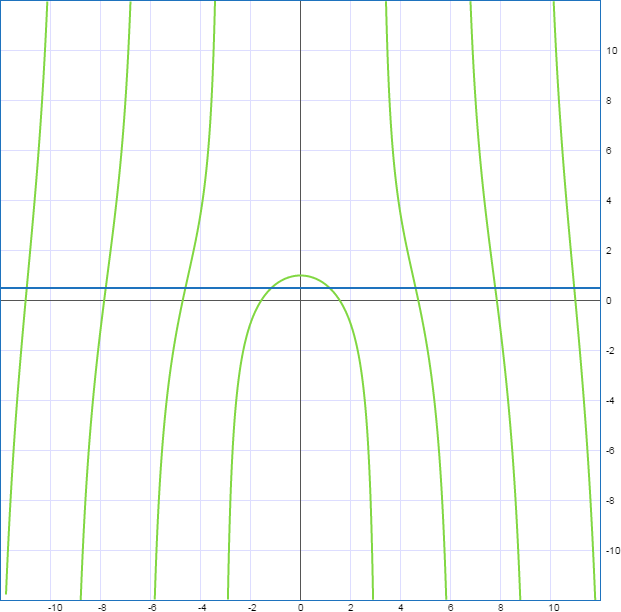
\includegraphics[scale=0.5]{xctg.png} 
\end{figure}

\end{frame}

\begin{frame}
\frametitle{ Critical value of $ \alpha $ } 

\begin{figure}
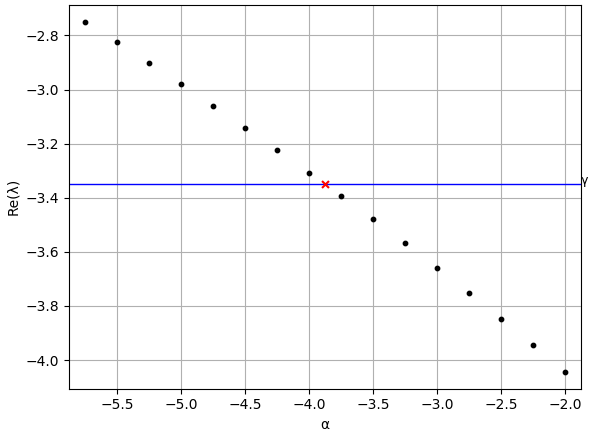
\includegraphics[scale=0.55]{Critical_alpha.png} 
\end{figure}
{\footnotesize $$ \gamma = -3.33 $$}

\end{frame}

\begin{frame}
\frametitle{ Plot } 

\begin{figure}
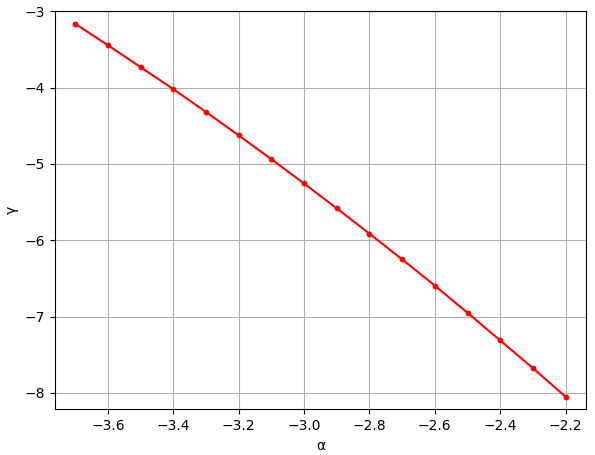
\includegraphics[scale=0.65]{Critical_relation.png} 
\end{figure}

\end{frame}

\begin{frame}
\frametitle{ Parabolic boundary-value problem } 

$$ u' = d \ddot{u} - \gamma u - u^3, $$

\bigskip

$$  u'\mid_{x=0} \, = 0, $$
$$ u'\mid_{x=1} \, = \alpha\,u\mid_{x=0}. $$

\end{frame}

\begin{frame}
\frametitle{ Dynamic system } 

\begin{eqnarray}\label{u_system} 
	\dot{u_j} = p^2(u_{j-1}-2u_j+u_{j+1}) - \gamma\,u_j - v_j^3, \qquad j=\overline{1,p},
\end{eqnarray}	

\bigskip

$$ u_0 = u_1, $$
$$ u_{p+1} = u_p + \frac{\alpha}{p}\,u_1. $$

\end{frame}

\begin{frame}
\frametitle{ Plot } 

\begin{figure}
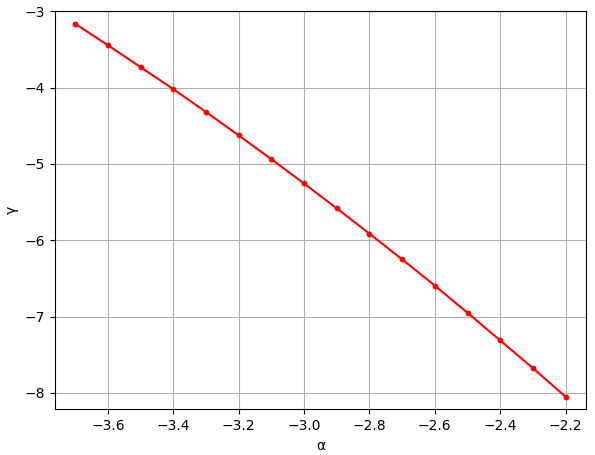
\includegraphics[scale=0.65]{Critical_relation.png}
\end{figure}

\end{frame}

\begin{frame}
\frametitle{ Andronov-Hopf bifurcation } 

\begin{figure}
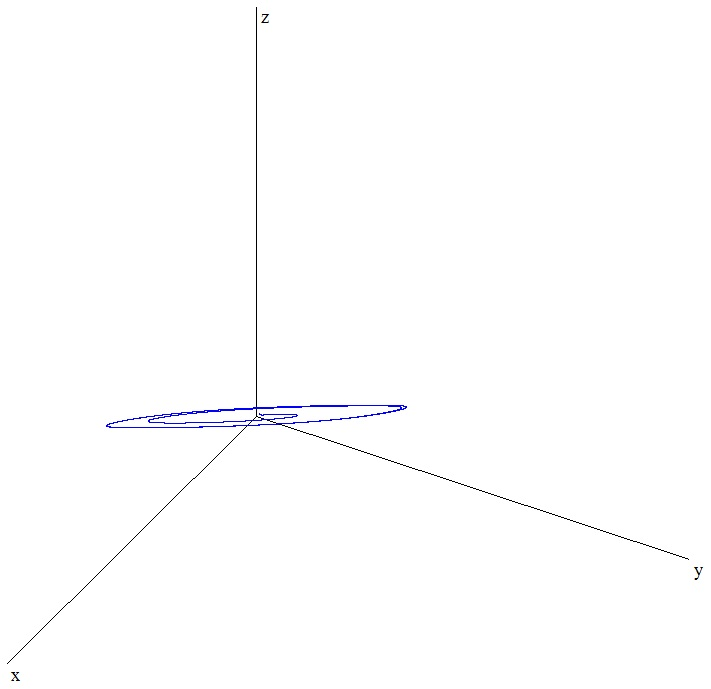
\includegraphics[scale=0.4]{AH.jpg} 
\end{figure}
{\footnotesize $$ \gamma = -5.58, \quad \alpha = -2.9 $$}

\end{frame}

\begin{frame}
\frametitle{ Andronov-Hopf bifurcation } 

\begin{figure}
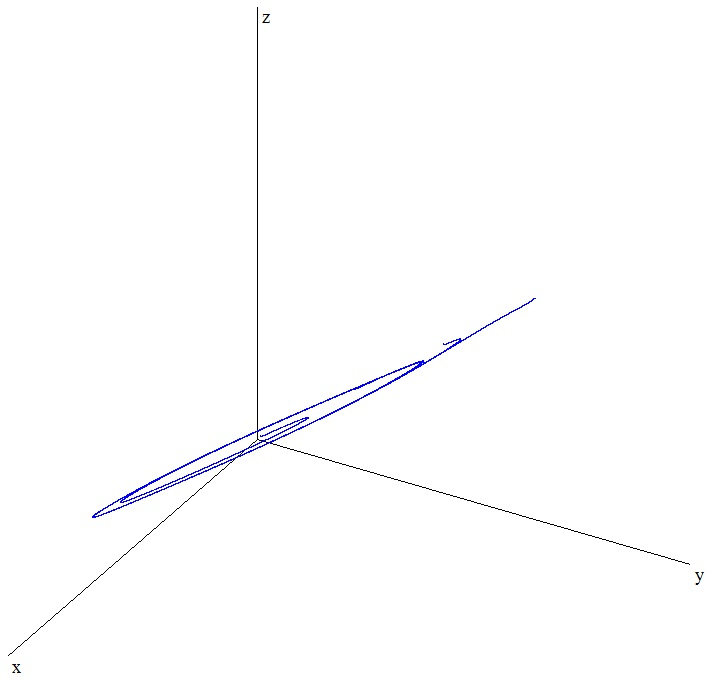
\includegraphics[scale=0.4]{AH2.jpg} 
\end{figure}
{\footnotesize $$ \gamma = -5.58, \quad \alpha = -2.9 $$}

\end{frame}

\end{document}